\documentclass{article}
\usepackage{amsfonts}
\usepackage[fleqn]{mathtools}
\usepackage{amssymb}
\usepackage[a4paper, total={6.5in, 9in}]{geometry}
\DeclareMathSizes{10}{10}{8}{8}
\hyphenpenalty=10000

\usepackage{graphicx}
\graphicspath{ {./pics/} }
\DeclareGraphicsExtensions{.jpg,.png}

\newcommand{\p}{\partial}
\newcommand{\fpd}[2][]{\frac{\partial #1}{\partial #2}}
\newcommand{\spd}[2][]{\frac{\partial^2 #1}{\partial #2}}
\newcommand{\hsp}[1][5]{\hspace{0.#1 cm}}
\newcommand{\hcm}[1][1]{\hspace{#1 cm}}
\newcommand{\bra}[1][1.2]{\scalebox{#1}{$\boldsymbol{\langle}$}}
\newcommand{\ket}[1][1.2]{\scalebox{#1}{$\boldsymbol{\rangle}$}}
\newcommand{\hh}{\hbar}
\newcommand{\dint}[4][0]{\int_{#1}^{#2} #3 \ d#4}
\newcommand{\lt}{\left}
\newcommand{\rt}{\right}
\newcommand{\lcm}{\text{lcm}}
\newcommand{\imp}{\Rightarrow}
\newcommand{\rimplies}{\Longleftarrow}
\newcommand{\rimp}{\Leftarrow}
\newcommand{\siff}{\Leftrightarrow}
\newcommand{\st}{\ : \ }

\newcommand{\N}{\mathbb{N}}
\newcommand{\Z}{\mathbb{Z}}
\newcommand{\Q}{\mathbb{Q}}
\newcommand{\R}{\mathbb{R}}
\newcommand{\C}{\mathbb{C}}
\newcommand{\G}[1][n]{\mathcal{G}_#1}
\newcommand{\POW}{\mathcal{P}}
\newcommand{\cat}{\mathsf{C}}
\newcommand{\HOM}{\text{Hom}}

\newcommand{\ch}[1]{\text{#1}}
\newcommand{\tdeg}{$^{\circ}$}
\newcommand{\mdeg}{^{\circ}}

\makeatletter
\newcommand*\bigcdot{\mathpalette\bigcdot@{.5}}
\newcommand*\bigcdot@[2]{\mathbin{\vcenter{\hbox{\scalebox{#2}{$\m@th#1\bullet$}}}}}
\makeatother
\newcommand{\inr}{{\mspace{2mu}\bigcdot\mspace{2mu}}}
\newcommand{\otr}{\raisebox{0.1ex}{\scalebox{0.7}{$\boldsymbol{\wedge}$}}}
\newcommand{\x}{{\times}}
\newcommand{\rev}{^\dag}
\newcommand{\nsubg}{\trianglelefteq}

\newcommand{\FLIPINDEX}[1]{{\scalebox{1}[-1]{$\scriptscriptstyle{#1}$}}}
\newcommand{\FLIPARG}[1]{{\scalebox{1}[-1]{$\mkern2mu#1$}}}


\newcommand{\dspt}{\displaystyle} 

\begin{document}
\begin{center}
algbra 0 aluffi
\end{center}
\begin{flushleft}
\textbf{note: I write function / morphism composition as $\mathbf{f(g(x)) = gf = f \circ g}$.}\\\ 

\hangindent=0.5cm 
2.5: $f$ is an epimorphism means $\forall a, b\ $ $fa=fb \imp a=b$.\\\ \\\hsp
Let $f:X\rightarrow Y$ be an epimorphism, and suppose it is not surjective, i.e. $\exists\ y \in Y$ with an empty fiber. Consider two maps $a,\ b$ from $Y$ to $\{0,1\}$: $a$ sends all of $Y$ to $0$, and $b$ is the same, except for sending $y \mapsto 1$. Then $fa = fb$ but $a \neq b$, so epimorphisms must be surjections.\\\ \\\hsp
Now let $f$ be surjective, i.e. every $y$ has a nonempty fiber $f_y$ (let $f(f_y)$ mean to pick an arbitrary $x\in f_y$ to put in $f$). Suppose for $a, b : Y \rightarrow Z$, $a\neq b$ but $fa = fb$.\\\hsp Then $\exists y\ a(y) \neq b(y) \imp a\circ f(f_y) \neq b\circ f(f_y)$, but we supposed $a \circ f = b \circ f$. The only way out was if $f_y$ was empty for some $y$, but $f$ is surjective. Hence $f$ surjective $\implies (fa = fb \imp a=b)$, i.e. $f$ is an epimorphism.\\\ 

2.9: Sets are isomorphic when they have the same cardinality. $A'\cap B' = \emptyset = A'' \cap B'' \iff |A' \cup B'| = |A'| + |B'| = |A''| + |B''| = |A'' \cup B''| \iff A' \cup B' \cong A'' \cup B''$.\\\ 

2.10: Each $a \in A$ has a choice of mapping to each $b \in B$. Since these choices are independent between different $a$'s, we multiply by $|B|$ for each $a \in A$, i.e. $|B^A| = |B|^{|A|}$\\\ 

2.11: A bijection is: $\forall p\in \POW(A)$, $\forall e\in A\ \ e\mapsto 1$ if $e \in P$, otherwise $e\mapsto 0$. Since a unique subset determines a unique map and vice-versa (construct the inverse), this is indeed a bijection.\\\ 

3.1: For $f \in \HOM_{\cat^{op}}(B,A)$ and $g \in \HOM_{\cat^{op}}(C,B)$, we define composition as $fg \in \HOM_{\cat^{op}}(C,A)$. This is well defined through the parent category: $f \in \HOM_\cat(A,B)$ and $g\in \HOM_\cat(B,C) \imp fg \in \HOM_\cat(A,C)$. Associativity and existence of the identity morphism also follow from the parent category.\\\ 

3.4: No, there is no identity.\\\ 

3.5: The $\subseteq$ relation is reflexive and transitive.\\\ 

3.6: finite dimensional vector spaces, the morphisms are maps between these spaces. A matrix with 0 rows/columns is a map involving $\vec{0}$.\\\ 

3.7: 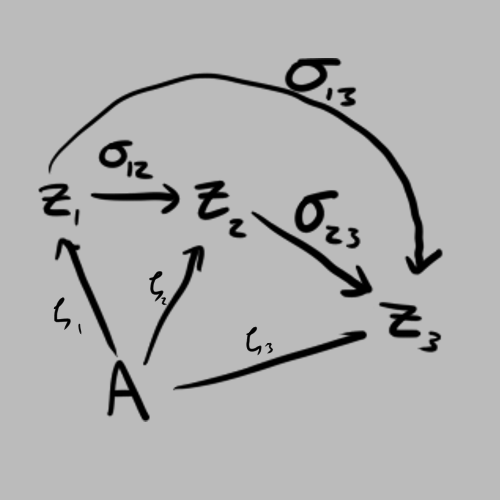
\includegraphics[height=4cm]{alg0-3-7} Elements of $\HOM(\zeta_1, \zeta_2)$ are morphisms $\sigma_{12}$ such that $\zeta_1\sigma_{12} = \zeta_2$. Composition is well-defined: $\zeta_1\sigma_{12}\sigma_{23} = \zeta_3 \imp \sigma_{12}\sigma_{23} = \sigma_{13} \in \HOM(\zeta_1,\zeta_3)$\\\ 

3.9: I think an isomorphism between msets should map equivalent elements to equivalent elements, with the objects of mset being a set equipped with an equivalence relation $\sim$. Generalizing, the morphisms are just functions where $a\sim b \imp f(a) \sim f(b)$, that way any morphism which is a bijection is an isomorphism. Set is a full subcategory as it is true for all functions that $a=b \imp f(a) = f(b)$.\\\ 

3.10: Any set with two elements is a subobject classifier in \textsf{Set}, with the subobjects being subsets.\\\  

3.11: 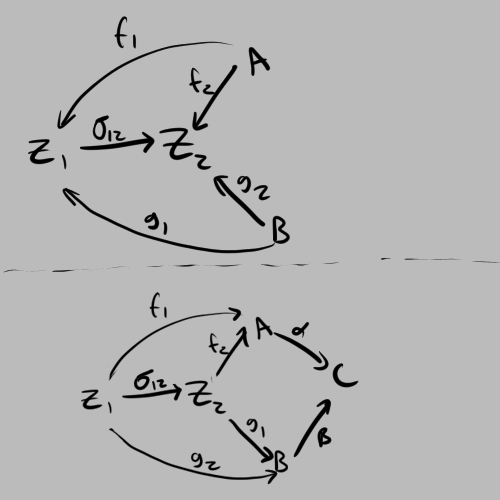
\includegraphics[height=4cm]{alg0-3-11}\\\hsp Note that the bottom category $\cat_{\alpha, \beta}$ ``looks like" a full subcategory of $\cat_{A,B}$, as in there is a one-to-one and onto mapping of objects and morphisms, respecting domain and composition, between $\cat_{\alpha, \beta}$ and a full subcategory of $\cat_{A,B}$.\\\ \\\hsp
For the top category $\cat^{A,B}$, we have $f_1\sigma_{12} = f_2$ and $g_1 \sigma_{12} = g_2$. \\\ 

4.1:
\end{flushleft}
\end{document}